\documentclass[twoside]{book}

% Packages required by doxygen
\usepackage{fixltx2e}
\usepackage{calc}
\usepackage{doxygen}
\usepackage[export]{adjustbox} % also loads graphicx
\usepackage{graphicx}
\usepackage[utf8]{inputenc}
\usepackage{makeidx}
\usepackage{multicol}
\usepackage{multirow}
\PassOptionsToPackage{warn}{textcomp}
\usepackage{textcomp}
\usepackage[nointegrals]{wasysym}
\usepackage[table]{xcolor}

% Font selection
\usepackage[T1]{fontenc}
\usepackage[scaled=.90]{helvet}
\usepackage{courier}
\usepackage{amssymb}
\usepackage{sectsty}
\renewcommand{\familydefault}{\sfdefault}
\allsectionsfont{%
  \fontseries{bc}\selectfont%
  \color{darkgray}%
}
\renewcommand{\DoxyLabelFont}{%
  \fontseries{bc}\selectfont%
  \color{darkgray}%
}
\newcommand{\+}{\discretionary{\mbox{\scriptsize$\hookleftarrow$}}{}{}}

% Page & text layout
\usepackage{geometry}
\geometry{%
  a4paper,%
  top=2.5cm,%
  bottom=2.5cm,%
  left=2.5cm,%
  right=2.5cm%
}
\tolerance=750
\hfuzz=15pt
\hbadness=750
\setlength{\emergencystretch}{15pt}
\setlength{\parindent}{0cm}
\setlength{\parskip}{3ex plus 2ex minus 2ex}
\makeatletter
\renewcommand{\paragraph}{%
  \@startsection{paragraph}{4}{0ex}{-1.0ex}{1.0ex}{%
    \normalfont\normalsize\bfseries\SS@parafont%
  }%
}
\renewcommand{\subparagraph}{%
  \@startsection{subparagraph}{5}{0ex}{-1.0ex}{1.0ex}{%
    \normalfont\normalsize\bfseries\SS@subparafont%
  }%
}
\makeatother

% Headers & footers
\usepackage{fancyhdr}
\pagestyle{fancyplain}
\fancyhead[LE]{\fancyplain{}{\bfseries\thepage}}
\fancyhead[CE]{\fancyplain{}{}}
\fancyhead[RE]{\fancyplain{}{\bfseries\leftmark}}
\fancyhead[LO]{\fancyplain{}{\bfseries\rightmark}}
\fancyhead[CO]{\fancyplain{}{}}
\fancyhead[RO]{\fancyplain{}{\bfseries\thepage}}
\fancyfoot[LE]{\fancyplain{}{}}
\fancyfoot[CE]{\fancyplain{}{}}
\fancyfoot[RE]{\fancyplain{}{\bfseries\scriptsize Generated by Doxygen }}
\fancyfoot[LO]{\fancyplain{}{\bfseries\scriptsize Generated by Doxygen }}
\fancyfoot[CO]{\fancyplain{}{}}
\fancyfoot[RO]{\fancyplain{}{}}
\renewcommand{\footrulewidth}{0.4pt}
\renewcommand{\chaptermark}[1]{%
  \markboth{#1}{}%
}
\renewcommand{\sectionmark}[1]{%
  \markright{\thesection\ #1}%
}

% Indices & bibliography
\usepackage{natbib}
\usepackage[titles]{tocloft}
\setcounter{tocdepth}{3}
\setcounter{secnumdepth}{5}
\makeindex

% Hyperlinks (required, but should be loaded last)
\usepackage{ifpdf}
\ifpdf
  \usepackage[pdftex,pagebackref=true]{hyperref}
\else
  \usepackage[ps2pdf,pagebackref=true]{hyperref}
\fi
\hypersetup{%
  colorlinks=true,%
  linkcolor=blue,%
  citecolor=blue,%
  unicode%
}

% Custom commands
\newcommand{\clearemptydoublepage}{%
  \newpage{\pagestyle{empty}\cleardoublepage}%
}

\usepackage{caption}
\captionsetup{labelsep=space,justification=centering,font={bf},singlelinecheck=off,skip=4pt,position=top}

%===== C O N T E N T S =====

\begin{document}

% Titlepage & ToC
\hypersetup{pageanchor=false,
             bookmarksnumbered=true,
             pdfencoding=unicode
            }
\pagenumbering{alph}
\begin{titlepage}
\vspace*{7cm}
\begin{center}%
{\Large My Project \\[1ex]\large 1 }\\
\vspace*{1cm}
{\large Generated by Doxygen 1.8.13}\\
\end{center}
\end{titlepage}
\clearemptydoublepage
\pagenumbering{roman}
\tableofcontents
\clearemptydoublepage
\pagenumbering{arabic}
\hypersetup{pageanchor=true}

%--- Begin generated contents ---
\chapter{Class Index}
\section{Class List}
Here are the classes, structs, unions and interfaces with brief descriptions\+:\begin{DoxyCompactList}
\item\contentsline{section}{\hyperlink{class_a_v_l_tree}{A\+V\+L\+Tree} \\*Class for A\+VL Tree }{\pageref{class_a_v_l_tree}}{}
\item\contentsline{section}{\hyperlink{structnode}{node} }{\pageref{structnode}}{}
\item\contentsline{section}{\hyperlink{class_node}{Node} }{\pageref{class_node}}{}
\item\contentsline{section}{\hyperlink{struct_r_b_t_node}{R\+B\+T\+Node} \\*\hyperlink{struct_r_b_t_node}{R\+B\+T\+Node} for red black tree }{\pageref{struct_r_b_t_node}}{}
\item\contentsline{section}{\hyperlink{class_r_b_tree}{R\+B\+Tree} \\*Class to represent Red-\/\+Black Tree }{\pageref{class_r_b_tree}}{}
\end{DoxyCompactList}

\chapter{File Index}
\section{File List}
Here is a list of all files with brief descriptions\+:\begin{DoxyCompactList}
\item\contentsline{section}{/home/kavya/\+Desktop/csn261\+\_\+lab\+\_\+assignment1/q1/code/\hyperlink{q1_8c}{q1.\+c} }{\pageref{q1_8c}}{}
\end{DoxyCompactList}

\chapter{Class Documentation}
\hypertarget{class_a_v_l_tree}{}\section{A\+V\+L\+Tree Class Reference}
\label{class_a_v_l_tree}\index{A\+V\+L\+Tree@{A\+V\+L\+Tree}}


Class for A\+VL Tree.  




Collaboration diagram for A\+V\+L\+Tree\+:
\nopagebreak
\begin{figure}[H]
\begin{center}
\leavevmode
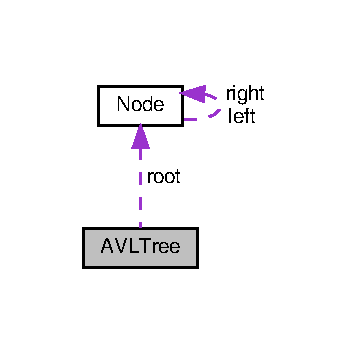
\includegraphics[width=168pt]{class_a_v_l_tree__coll__graph}
\end{center}
\end{figure}
\subsection*{Public Member Functions}
\begin{DoxyCompactItemize}
\item 
int \hyperlink{class_a_v_l_tree_a96cbfc11d7b61204423d22d4dec3cb39}{height} (\hyperlink{class_node}{Node} $\ast$N)
\item 
int \hyperlink{class_a_v_l_tree_ae5cd885ee0ad8a06a933bdac473c3cc5}{max} (int a, int b)
\item 
\hyperlink{class_node}{Node} $\ast$ \hyperlink{class_a_v_l_tree_a7d0da3880ea6b30f7df37547f99be642}{new\+Node} (int key)
\item 
\hyperlink{class_node}{Node} $\ast$ \hyperlink{class_a_v_l_tree_a735406d043d3dc61e0ed08455381487a}{right\+Rotate} (\hyperlink{class_node}{Node} $\ast$y)
\item 
\hyperlink{class_node}{Node} $\ast$ \hyperlink{class_a_v_l_tree_a8dc98844f7c4301e071bbc7c062ba9b5}{left\+Rotate} (\hyperlink{class_node}{Node} $\ast$x)
\item 
int \hyperlink{class_a_v_l_tree_aff1b11f5d1e3b013877c1fc1ace0b6a8}{get\+Balance} (\hyperlink{class_node}{Node} $\ast$N)
\item 
\hyperlink{class_node}{Node} $\ast$ \hyperlink{class_a_v_l_tree_adab09466d7b80c7b10eade93fca1b831}{insert} (\hyperlink{class_node}{Node} $\ast$\hyperlink{structnode}{node}, int key)
\item 
void \hyperlink{class_a_v_l_tree_a3dc3f18fce5d4124bfb94eb6cfa2e400}{in\+Order} (\hyperlink{class_node}{Node} $\ast$\hyperlink{class_a_v_l_tree_a3db9914a012a92648fc774b1112c79f0}{root})
\item 
void \hyperlink{class_a_v_l_tree_a4a917504798c964c12d6ea23bff6710c}{level\+Vise\+Indentation\+Helper} (\hyperlink{class_node}{Node} $\ast$rt, int l)
\item 
void \hyperlink{class_a_v_l_tree_a4717d25b108d9ad8d67258c75e44f696}{level\+Vise\+Indentation} ()
\item 
void \hyperlink{class_a_v_l_tree_a6fe238e7e0e458de06ee3357f5044e3a}{print\+Path} (\hyperlink{class_node}{Node} $\ast$rt, string s)
\item 
void \hyperlink{class_a_v_l_tree_acfeb6a8c2b2ddd309747a7f5d402e2ed}{get\+All\+Paths} ()
\end{DoxyCompactItemize}
\subsection*{Public Attributes}
\begin{DoxyCompactItemize}
\item 
\hyperlink{class_node}{Node} $\ast$ \hyperlink{class_a_v_l_tree_a3db9914a012a92648fc774b1112c79f0}{root}
\begin{DoxyCompactList}\small\item\em Root of A\+VL Tree. \end{DoxyCompactList}\end{DoxyCompactItemize}


\subsection{Detailed Description}
Class for A\+VL Tree. 

Definition at line 368 of file q1.\+cpp.



\subsection{Member Function Documentation}
\mbox{\Hypertarget{class_a_v_l_tree_acfeb6a8c2b2ddd309747a7f5d402e2ed}\label{class_a_v_l_tree_acfeb6a8c2b2ddd309747a7f5d402e2ed}} 
\index{A\+V\+L\+Tree@{A\+V\+L\+Tree}!get\+All\+Paths@{get\+All\+Paths}}
\index{get\+All\+Paths@{get\+All\+Paths}!A\+V\+L\+Tree@{A\+V\+L\+Tree}}
\subsubsection{\texorpdfstring{get\+All\+Paths()}{getAllPaths()}}
{\footnotesize\ttfamily void A\+V\+L\+Tree\+::get\+All\+Paths (\begin{DoxyParamCaption}{ }\end{DoxyParamCaption})\hspace{0.3cm}{\ttfamily [inline]}}

This method will be used to print all the paths from root node to the N\+U\+LL pointers of A\+VL Tree. \begin{DoxyAuthor}{Author}
Kavya Barnwal 
\end{DoxyAuthor}
\begin{DoxyDate}{Date}
20/08/2019 
\end{DoxyDate}


Definition at line 616 of file q1.\+cpp.

\mbox{\Hypertarget{class_a_v_l_tree_aff1b11f5d1e3b013877c1fc1ace0b6a8}\label{class_a_v_l_tree_aff1b11f5d1e3b013877c1fc1ace0b6a8}} 
\index{A\+V\+L\+Tree@{A\+V\+L\+Tree}!get\+Balance@{get\+Balance}}
\index{get\+Balance@{get\+Balance}!A\+V\+L\+Tree@{A\+V\+L\+Tree}}
\subsubsection{\texorpdfstring{get\+Balance()}{getBalance()}}
{\footnotesize\ttfamily int A\+V\+L\+Tree\+::get\+Balance (\begin{DoxyParamCaption}\item[{\hyperlink{class_node}{Node} $\ast$}]{N }\end{DoxyParamCaption})\hspace{0.3cm}{\ttfamily [inline]}}

Get Balance factor of node N. 
\begin{DoxyParams}{Parameters}
{\em N} & \hyperlink{class_node}{Node} for which balance factor is to be determined. \\
\hline
\end{DoxyParams}
\begin{DoxyAuthor}{Author}
Kavya Barnwal 
\end{DoxyAuthor}
\begin{DoxyDate}{Date}
20/08/2019 
\end{DoxyDate}


Definition at line 476 of file q1.\+cpp.

\mbox{\Hypertarget{class_a_v_l_tree_a96cbfc11d7b61204423d22d4dec3cb39}\label{class_a_v_l_tree_a96cbfc11d7b61204423d22d4dec3cb39}} 
\index{A\+V\+L\+Tree@{A\+V\+L\+Tree}!height@{height}}
\index{height@{height}!A\+V\+L\+Tree@{A\+V\+L\+Tree}}
\subsubsection{\texorpdfstring{height()}{height()}}
{\footnotesize\ttfamily int A\+V\+L\+Tree\+::height (\begin{DoxyParamCaption}\item[{\hyperlink{class_node}{Node} $\ast$}]{N }\end{DoxyParamCaption})\hspace{0.3cm}{\ttfamily [inline]}}

A utility function to get the height of the tree. 
\begin{DoxyParams}{Parameters}
{\em N} & \hyperlink{class_node}{Node} of which height to be determined \\
\hline
\end{DoxyParams}
\begin{DoxyAuthor}{Author}
Kavya Barnwal 
\end{DoxyAuthor}
\begin{DoxyDate}{Date}
20/08/2019 
\end{DoxyDate}


Definition at line 380 of file q1.\+cpp.

\mbox{\Hypertarget{class_a_v_l_tree_a3dc3f18fce5d4124bfb94eb6cfa2e400}\label{class_a_v_l_tree_a3dc3f18fce5d4124bfb94eb6cfa2e400}} 
\index{A\+V\+L\+Tree@{A\+V\+L\+Tree}!in\+Order@{in\+Order}}
\index{in\+Order@{in\+Order}!A\+V\+L\+Tree@{A\+V\+L\+Tree}}
\subsubsection{\texorpdfstring{in\+Order()}{inOrder()}}
{\footnotesize\ttfamily void A\+V\+L\+Tree\+::in\+Order (\begin{DoxyParamCaption}\item[{\hyperlink{class_node}{Node} $\ast$}]{root }\end{DoxyParamCaption})\hspace{0.3cm}{\ttfamily [inline]}}

A utility function to print preorder traversal of the tree. The function also prints height of every node. 
\begin{DoxyParams}{Parameters}
{\em root} & Root of A\+VL Tree. \\
\hline
\end{DoxyParams}
\begin{DoxyAuthor}{Author}
Kavya Barnwal 
\end{DoxyAuthor}
\begin{DoxyDate}{Date}
20/08/2019 
\end{DoxyDate}


Definition at line 547 of file q1.\+cpp.

\mbox{\Hypertarget{class_a_v_l_tree_adab09466d7b80c7b10eade93fca1b831}\label{class_a_v_l_tree_adab09466d7b80c7b10eade93fca1b831}} 
\index{A\+V\+L\+Tree@{A\+V\+L\+Tree}!insert@{insert}}
\index{insert@{insert}!A\+V\+L\+Tree@{A\+V\+L\+Tree}}
\subsubsection{\texorpdfstring{insert()}{insert()}}
{\footnotesize\ttfamily \hyperlink{class_node}{Node}$\ast$ A\+V\+L\+Tree\+::insert (\begin{DoxyParamCaption}\item[{\hyperlink{class_node}{Node} $\ast$}]{node,  }\item[{int}]{key }\end{DoxyParamCaption})\hspace{0.3cm}{\ttfamily [inline]}}

Recursive function to insert a key in the subtree rooted with node and returns the new root of the subtree. 
\begin{DoxyParams}{Parameters}
{\em node} & Root of A\+VL Tree. \\
\hline
{\em data} & integer to be inserted. \\
\hline
\end{DoxyParams}
\begin{DoxyAuthor}{Author}
Kavya Barnwal 
\end{DoxyAuthor}
\begin{DoxyDate}{Date}
20/08/2019 
\end{DoxyDate}


Definition at line 490 of file q1.\+cpp.

\mbox{\Hypertarget{class_a_v_l_tree_a8dc98844f7c4301e071bbc7c062ba9b5}\label{class_a_v_l_tree_a8dc98844f7c4301e071bbc7c062ba9b5}} 
\index{A\+V\+L\+Tree@{A\+V\+L\+Tree}!left\+Rotate@{left\+Rotate}}
\index{left\+Rotate@{left\+Rotate}!A\+V\+L\+Tree@{A\+V\+L\+Tree}}
\subsubsection{\texorpdfstring{left\+Rotate()}{leftRotate()}}
{\footnotesize\ttfamily \hyperlink{class_node}{Node}$\ast$ A\+V\+L\+Tree\+::left\+Rotate (\begin{DoxyParamCaption}\item[{\hyperlink{class_node}{Node} $\ast$}]{x }\end{DoxyParamCaption})\hspace{0.3cm}{\ttfamily [inline]}}

A utility function to left rotate subtree rooted with y. 
\begin{DoxyParams}{Parameters}
{\em x} & \hyperlink{class_node}{Node} about which to be rotated. \\
\hline
\end{DoxyParams}
\begin{DoxyAuthor}{Author}
Kavya Barnwal 
\end{DoxyAuthor}
\begin{DoxyDate}{Date}
20/08/2019 
\end{DoxyDate}


Definition at line 449 of file q1.\+cpp.

\mbox{\Hypertarget{class_a_v_l_tree_a4717d25b108d9ad8d67258c75e44f696}\label{class_a_v_l_tree_a4717d25b108d9ad8d67258c75e44f696}} 
\index{A\+V\+L\+Tree@{A\+V\+L\+Tree}!level\+Vise\+Indentation@{level\+Vise\+Indentation}}
\index{level\+Vise\+Indentation@{level\+Vise\+Indentation}!A\+V\+L\+Tree@{A\+V\+L\+Tree}}
\subsubsection{\texorpdfstring{level\+Vise\+Indentation()}{levelViseIndentation()}}
{\footnotesize\ttfamily void A\+V\+L\+Tree\+::level\+Vise\+Indentation (\begin{DoxyParamCaption}{ }\end{DoxyParamCaption})\hspace{0.3cm}{\ttfamily [inline]}}

This method will be used to print the A\+VL Tree with lavel-\/wise-\/indentation. \begin{DoxyAuthor}{Author}
Kavya Barnwal 
\end{DoxyAuthor}
\begin{DoxyDate}{Date}
20/08/2019 
\end{DoxyDate}


Definition at line 584 of file q1.\+cpp.

\mbox{\Hypertarget{class_a_v_l_tree_a4a917504798c964c12d6ea23bff6710c}\label{class_a_v_l_tree_a4a917504798c964c12d6ea23bff6710c}} 
\index{A\+V\+L\+Tree@{A\+V\+L\+Tree}!level\+Vise\+Indentation\+Helper@{level\+Vise\+Indentation\+Helper}}
\index{level\+Vise\+Indentation\+Helper@{level\+Vise\+Indentation\+Helper}!A\+V\+L\+Tree@{A\+V\+L\+Tree}}
\subsubsection{\texorpdfstring{level\+Vise\+Indentation\+Helper()}{levelViseIndentationHelper()}}
{\footnotesize\ttfamily void A\+V\+L\+Tree\+::level\+Vise\+Indentation\+Helper (\begin{DoxyParamCaption}\item[{\hyperlink{class_node}{Node} $\ast$}]{rt,  }\item[{int}]{l }\end{DoxyParamCaption})\hspace{0.3cm}{\ttfamily [inline]}}

Helper method for method \hyperlink{class_a_v_l_tree_a4717d25b108d9ad8d67258c75e44f696}{level\+Vise\+Indentation()}. 
\begin{DoxyParams}{Parameters}
{\em root} & Root of A\+VL Tree. \\
\hline
{\em l} & level of that node. \\
\hline
\end{DoxyParams}
\begin{DoxyAuthor}{Author}
Kavya Barnwal 
\end{DoxyAuthor}
\begin{DoxyDate}{Date}
20/08/2019 
\end{DoxyDate}


Definition at line 564 of file q1.\+cpp.

\mbox{\Hypertarget{class_a_v_l_tree_ae5cd885ee0ad8a06a933bdac473c3cc5}\label{class_a_v_l_tree_ae5cd885ee0ad8a06a933bdac473c3cc5}} 
\index{A\+V\+L\+Tree@{A\+V\+L\+Tree}!max@{max}}
\index{max@{max}!A\+V\+L\+Tree@{A\+V\+L\+Tree}}
\subsubsection{\texorpdfstring{max()}{max()}}
{\footnotesize\ttfamily int A\+V\+L\+Tree\+::max (\begin{DoxyParamCaption}\item[{int}]{a,  }\item[{int}]{b }\end{DoxyParamCaption})\hspace{0.3cm}{\ttfamily [inline]}}

A utility function to get maximum of two integers. 
\begin{DoxyParams}{Parameters}
{\em a} & first integer. \\
\hline
{\em b} & second integer. \\
\hline
\end{DoxyParams}
\begin{DoxyAuthor}{Author}
Kavya Barnwal 
\end{DoxyAuthor}
\begin{DoxyDate}{Date}
20/08/2019 
\end{DoxyDate}


Definition at line 394 of file q1.\+cpp.

\mbox{\Hypertarget{class_a_v_l_tree_a7d0da3880ea6b30f7df37547f99be642}\label{class_a_v_l_tree_a7d0da3880ea6b30f7df37547f99be642}} 
\index{A\+V\+L\+Tree@{A\+V\+L\+Tree}!new\+Node@{new\+Node}}
\index{new\+Node@{new\+Node}!A\+V\+L\+Tree@{A\+V\+L\+Tree}}
\subsubsection{\texorpdfstring{new\+Node()}{newNode()}}
{\footnotesize\ttfamily \hyperlink{class_node}{Node}$\ast$ A\+V\+L\+Tree\+::new\+Node (\begin{DoxyParamCaption}\item[{int}]{key }\end{DoxyParamCaption})\hspace{0.3cm}{\ttfamily [inline]}}

Helper function that allocates a new node with the given key and N\+U\+LL left and right pointers. 
\begin{DoxyParams}{Parameters}
{\em key} & data to be inserted. \\
\hline
\end{DoxyParams}
\begin{DoxyAuthor}{Author}
Kavya Barnwal 
\end{DoxyAuthor}
\begin{DoxyDate}{Date}
20/08/2019 
\end{DoxyDate}


Definition at line 405 of file q1.\+cpp.

\mbox{\Hypertarget{class_a_v_l_tree_a6fe238e7e0e458de06ee3357f5044e3a}\label{class_a_v_l_tree_a6fe238e7e0e458de06ee3357f5044e3a}} 
\index{A\+V\+L\+Tree@{A\+V\+L\+Tree}!print\+Path@{print\+Path}}
\index{print\+Path@{print\+Path}!A\+V\+L\+Tree@{A\+V\+L\+Tree}}
\subsubsection{\texorpdfstring{print\+Path()}{printPath()}}
{\footnotesize\ttfamily void A\+V\+L\+Tree\+::print\+Path (\begin{DoxyParamCaption}\item[{\hyperlink{class_node}{Node} $\ast$}]{rt,  }\item[{string}]{s }\end{DoxyParamCaption})\hspace{0.3cm}{\ttfamily [inline]}}

Helper method for method \hyperlink{class_a_v_l_tree_acfeb6a8c2b2ddd309747a7f5d402e2ed}{get\+All\+Paths()}. 
\begin{DoxyParams}{Parameters}
{\em rt} & Root of A\+VL Tree. \\
\hline
{\em s} & string containing details of nodes traversed. \\
\hline
\end{DoxyParams}
\begin{DoxyAuthor}{Author}
Kavya Barnwal 
\end{DoxyAuthor}
\begin{DoxyDate}{Date}
20/08/2019 
\end{DoxyDate}


Definition at line 595 of file q1.\+cpp.

\mbox{\Hypertarget{class_a_v_l_tree_a735406d043d3dc61e0ed08455381487a}\label{class_a_v_l_tree_a735406d043d3dc61e0ed08455381487a}} 
\index{A\+V\+L\+Tree@{A\+V\+L\+Tree}!right\+Rotate@{right\+Rotate}}
\index{right\+Rotate@{right\+Rotate}!A\+V\+L\+Tree@{A\+V\+L\+Tree}}
\subsubsection{\texorpdfstring{right\+Rotate()}{rightRotate()}}
{\footnotesize\ttfamily \hyperlink{class_node}{Node}$\ast$ A\+V\+L\+Tree\+::right\+Rotate (\begin{DoxyParamCaption}\item[{\hyperlink{class_node}{Node} $\ast$}]{y }\end{DoxyParamCaption})\hspace{0.3cm}{\ttfamily [inline]}}

A utility function to right rotate subtree rooted with y. 
\begin{DoxyParams}{Parameters}
{\em y} & \hyperlink{class_node}{Node} about which to be rotated. \\
\hline
\end{DoxyParams}
\begin{DoxyAuthor}{Author}
Kavya Barnwal 
\end{DoxyAuthor}
\begin{DoxyDate}{Date}
20/08/2019 
\end{DoxyDate}


Definition at line 422 of file q1.\+cpp.



\subsection{Member Data Documentation}
\mbox{\Hypertarget{class_a_v_l_tree_a3db9914a012a92648fc774b1112c79f0}\label{class_a_v_l_tree_a3db9914a012a92648fc774b1112c79f0}} 
\index{A\+V\+L\+Tree@{A\+V\+L\+Tree}!root@{root}}
\index{root@{root}!A\+V\+L\+Tree@{A\+V\+L\+Tree}}
\subsubsection{\texorpdfstring{root}{root}}
{\footnotesize\ttfamily \hyperlink{class_node}{Node}$\ast$ A\+V\+L\+Tree\+::root}



Root of A\+VL Tree. 



Definition at line 372 of file q1.\+cpp.



The documentation for this class was generated from the following file\+:\begin{DoxyCompactItemize}
\item 
/home/kavya/\+Desktop/ass3/q1/code/\hyperlink{q1_8cpp}{q1.\+cpp}\end{DoxyCompactItemize}

\hypertarget{structnode}{}\section{node$<$ V $>$ Struct Template Reference}
\label{structnode}\index{node$<$ V $>$@{node$<$ V $>$}}


{\ttfamily \#include $<$fibonacci\+\_\+heap.\+h$>$}

\subsection*{Public Attributes}
\begin{DoxyCompactItemize}
\item 
\hyperlink{structnode}{node}$<$ V $>$ $\ast$ \hyperlink{structnode_a203e6d9b472c65ef97d3acd4b961b301}{prev}
\item 
\hyperlink{structnode}{node}$<$ V $>$ $\ast$ \hyperlink{structnode_a5c15f160b3b242d1ee025bdb67c9c798}{next}
\item 
\hyperlink{structnode}{node}$<$ V $>$ $\ast$ \hyperlink{structnode_a4b6a5eded3c2188e96413a620a748d83}{child}
\item 
\hyperlink{structnode}{node}$<$ V $>$ $\ast$ \hyperlink{structnode_afb2d1d451cf8cea46087ce30258499ca}{parent}
\item 
V \hyperlink{structnode_a1a2d957a20bcdfbf21dcb73e2378a5ea}{value}
\item 
int \hyperlink{structnode_ab9c3a691bf0c39288401ae0056b6b0cc}{degree}
\item 
bool \hyperlink{structnode_a6800b687c66c2087c17d541af91184ff}{marked}
\end{DoxyCompactItemize}


\subsection{Detailed Description}
\subsubsection*{template$<$class V$>$\newline
struct node$<$ V $>$}



Definition at line 3 of file fibonacci\+\_\+heap.\+h.



\subsection{Member Data Documentation}
\mbox{\Hypertarget{structnode_a4b6a5eded3c2188e96413a620a748d83}\label{structnode_a4b6a5eded3c2188e96413a620a748d83}} 
\index{node@{node}!child@{child}}
\index{child@{child}!node@{node}}
\subsubsection{\texorpdfstring{child}{child}}
{\footnotesize\ttfamily template$<$class V$>$ \\
\hyperlink{structnode}{node}$<$V$>$$\ast$ \hyperlink{structnode}{node}$<$ V $>$\+::child}



Definition at line 8 of file fibonacci\+\_\+heap.\+h.

\mbox{\Hypertarget{structnode_ab9c3a691bf0c39288401ae0056b6b0cc}\label{structnode_ab9c3a691bf0c39288401ae0056b6b0cc}} 
\index{node@{node}!degree@{degree}}
\index{degree@{degree}!node@{node}}
\subsubsection{\texorpdfstring{degree}{degree}}
{\footnotesize\ttfamily template$<$class V$>$ \\
int \hyperlink{structnode}{node}$<$ V $>$\+::degree}



Definition at line 11 of file fibonacci\+\_\+heap.\+h.

\mbox{\Hypertarget{structnode_a6800b687c66c2087c17d541af91184ff}\label{structnode_a6800b687c66c2087c17d541af91184ff}} 
\index{node@{node}!marked@{marked}}
\index{marked@{marked}!node@{node}}
\subsubsection{\texorpdfstring{marked}{marked}}
{\footnotesize\ttfamily template$<$class V$>$ \\
bool \hyperlink{structnode}{node}$<$ V $>$\+::marked}



Definition at line 12 of file fibonacci\+\_\+heap.\+h.

\mbox{\Hypertarget{structnode_a5c15f160b3b242d1ee025bdb67c9c798}\label{structnode_a5c15f160b3b242d1ee025bdb67c9c798}} 
\index{node@{node}!next@{next}}
\index{next@{next}!node@{node}}
\subsubsection{\texorpdfstring{next}{next}}
{\footnotesize\ttfamily template$<$class V$>$ \\
\hyperlink{structnode}{node}$<$V$>$$\ast$ \hyperlink{structnode}{node}$<$ V $>$\+::next}



Definition at line 7 of file fibonacci\+\_\+heap.\+h.

\mbox{\Hypertarget{structnode_afb2d1d451cf8cea46087ce30258499ca}\label{structnode_afb2d1d451cf8cea46087ce30258499ca}} 
\index{node@{node}!parent@{parent}}
\index{parent@{parent}!node@{node}}
\subsubsection{\texorpdfstring{parent}{parent}}
{\footnotesize\ttfamily template$<$class V$>$ \\
\hyperlink{structnode}{node}$<$V$>$$\ast$ \hyperlink{structnode}{node}$<$ V $>$\+::parent}



Definition at line 9 of file fibonacci\+\_\+heap.\+h.

\mbox{\Hypertarget{structnode_a203e6d9b472c65ef97d3acd4b961b301}\label{structnode_a203e6d9b472c65ef97d3acd4b961b301}} 
\index{node@{node}!prev@{prev}}
\index{prev@{prev}!node@{node}}
\subsubsection{\texorpdfstring{prev}{prev}}
{\footnotesize\ttfamily template$<$class V$>$ \\
\hyperlink{structnode}{node}$<$V$>$$\ast$ \hyperlink{structnode}{node}$<$ V $>$\+::prev}



Definition at line 6 of file fibonacci\+\_\+heap.\+h.

\mbox{\Hypertarget{structnode_a1a2d957a20bcdfbf21dcb73e2378a5ea}\label{structnode_a1a2d957a20bcdfbf21dcb73e2378a5ea}} 
\index{node@{node}!value@{value}}
\index{value@{value}!node@{node}}
\subsubsection{\texorpdfstring{value}{value}}
{\footnotesize\ttfamily template$<$class V$>$ \\
V \hyperlink{structnode}{node}$<$ V $>$\+::value}



Definition at line 10 of file fibonacci\+\_\+heap.\+h.



The documentation for this struct was generated from the following file\+:\begin{DoxyCompactItemize}
\item 
code/\hyperlink{fibonacci__heap_8h}{fibonacci\+\_\+heap.\+h}\end{DoxyCompactItemize}

\hypertarget{class_node}{}\section{Node Class Reference}
\label{class_node}\index{Node@{Node}}


Collaboration diagram for Node\+:
\nopagebreak
\begin{figure}[H]
\begin{center}
\leavevmode
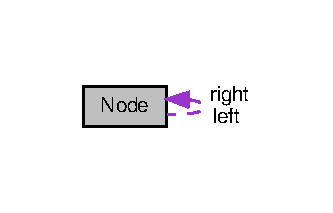
\includegraphics[width=160pt]{class_node__coll__graph}
\end{center}
\end{figure}
\subsection*{Public Attributes}
\begin{DoxyCompactItemize}
\item 
int \hyperlink{class_node_a3020957813f200a9da836428aad2d8d7}{key}
\item 
\hyperlink{class_node}{Node} $\ast$ \hyperlink{class_node_ab8c667ac8fdb120ed4c031682a9cdaee}{left}
\item 
\hyperlink{class_node}{Node} $\ast$ \hyperlink{class_node_a7328862eaa6dea28018326549b3294d3}{right}
\item 
int \hyperlink{class_node_a61966b207f0584aaa4773e5e1266e905}{height}
\end{DoxyCompactItemize}


\subsection{Detailed Description}


Definition at line 358 of file q1.\+cpp.



\subsection{Member Data Documentation}
\mbox{\Hypertarget{class_node_a61966b207f0584aaa4773e5e1266e905}\label{class_node_a61966b207f0584aaa4773e5e1266e905}} 
\index{Node@{Node}!height@{height}}
\index{height@{height}!Node@{Node}}
\subsubsection{\texorpdfstring{height}{height}}
{\footnotesize\ttfamily int Node\+::height}



Definition at line 364 of file q1.\+cpp.

\mbox{\Hypertarget{class_node_a3020957813f200a9da836428aad2d8d7}\label{class_node_a3020957813f200a9da836428aad2d8d7}} 
\index{Node@{Node}!key@{key}}
\index{key@{key}!Node@{Node}}
\subsubsection{\texorpdfstring{key}{key}}
{\footnotesize\ttfamily int Node\+::key}



Definition at line 361 of file q1.\+cpp.

\mbox{\Hypertarget{class_node_ab8c667ac8fdb120ed4c031682a9cdaee}\label{class_node_ab8c667ac8fdb120ed4c031682a9cdaee}} 
\index{Node@{Node}!left@{left}}
\index{left@{left}!Node@{Node}}
\subsubsection{\texorpdfstring{left}{left}}
{\footnotesize\ttfamily \hyperlink{class_node}{Node}$\ast$ Node\+::left}



Definition at line 362 of file q1.\+cpp.

\mbox{\Hypertarget{class_node_a7328862eaa6dea28018326549b3294d3}\label{class_node_a7328862eaa6dea28018326549b3294d3}} 
\index{Node@{Node}!right@{right}}
\index{right@{right}!Node@{Node}}
\subsubsection{\texorpdfstring{right}{right}}
{\footnotesize\ttfamily \hyperlink{class_node}{Node}$\ast$ Node\+::right}



Definition at line 363 of file q1.\+cpp.



The documentation for this class was generated from the following file\+:\begin{DoxyCompactItemize}
\item 
/home/kavya/\+Desktop/ass3/q1/code/\hyperlink{q1_8cpp}{q1.\+cpp}\end{DoxyCompactItemize}

\hypertarget{struct_r_b_t_node}{}\section{R\+B\+T\+Node Struct Reference}
\label{struct_r_b_t_node}\index{R\+B\+T\+Node@{R\+B\+T\+Node}}


\hyperlink{struct_r_b_t_node}{R\+B\+T\+Node} for red black tree.  




Collaboration diagram for R\+B\+T\+Node\+:
\nopagebreak
\begin{figure}[H]
\begin{center}
\leavevmode
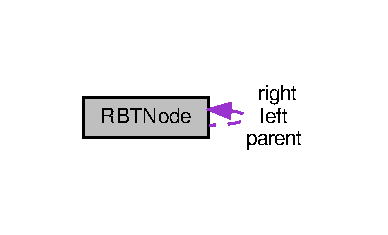
\includegraphics[width=186pt]{struct_r_b_t_node__coll__graph}
\end{center}
\end{figure}
\subsection*{Public Member Functions}
\begin{DoxyCompactItemize}
\item 
\hyperlink{struct_r_b_t_node_a0392480d9b347b937fed779ebfba204b}{R\+B\+T\+Node} (int \hyperlink{struct_r_b_t_node_a3d765df58677c77bf9e3743938d41d0d}{data})
\begin{DoxyCompactList}\small\item\em Constructor. \end{DoxyCompactList}\end{DoxyCompactItemize}
\subsection*{Public Attributes}
\begin{DoxyCompactItemize}
\item 
int \hyperlink{struct_r_b_t_node_a3d765df58677c77bf9e3743938d41d0d}{data}
\item 
bool \hyperlink{struct_r_b_t_node_a8e8fa974e4586ceb0883861952fde8e0}{color}
\item 
\hyperlink{struct_r_b_t_node}{R\+B\+T\+Node} $\ast$ \hyperlink{struct_r_b_t_node_ab365a258e6d393e3a2b1b876a72b57b8}{left}
\item 
\hyperlink{struct_r_b_t_node}{R\+B\+T\+Node} $\ast$ \hyperlink{struct_r_b_t_node_a56bcde7ab9200c37bcbeb736b7b3cd06}{right}
\item 
\hyperlink{struct_r_b_t_node}{R\+B\+T\+Node} $\ast$ \hyperlink{struct_r_b_t_node_accf38a2652c418128932b2f13283ba8c}{parent}
\end{DoxyCompactItemize}


\subsection{Detailed Description}
\hyperlink{struct_r_b_t_node}{R\+B\+T\+Node} for red black tree. 

Definition at line 13 of file q1.\+cpp.



\subsection{Constructor \& Destructor Documentation}
\mbox{\Hypertarget{struct_r_b_t_node_a0392480d9b347b937fed779ebfba204b}\label{struct_r_b_t_node_a0392480d9b347b937fed779ebfba204b}} 
\index{R\+B\+T\+Node@{R\+B\+T\+Node}!R\+B\+T\+Node@{R\+B\+T\+Node}}
\index{R\+B\+T\+Node@{R\+B\+T\+Node}!R\+B\+T\+Node@{R\+B\+T\+Node}}
\subsubsection{\texorpdfstring{R\+B\+T\+Node()}{RBTNode()}}
{\footnotesize\ttfamily R\+B\+T\+Node\+::\+R\+B\+T\+Node (\begin{DoxyParamCaption}\item[{int}]{data }\end{DoxyParamCaption})\hspace{0.3cm}{\ttfamily [inline]}}



Constructor. 



Definition at line 20 of file q1.\+cpp.



\subsection{Member Data Documentation}
\mbox{\Hypertarget{struct_r_b_t_node_a8e8fa974e4586ceb0883861952fde8e0}\label{struct_r_b_t_node_a8e8fa974e4586ceb0883861952fde8e0}} 
\index{R\+B\+T\+Node@{R\+B\+T\+Node}!color@{color}}
\index{color@{color}!R\+B\+T\+Node@{R\+B\+T\+Node}}
\subsubsection{\texorpdfstring{color}{color}}
{\footnotesize\ttfamily bool R\+B\+T\+Node\+::color}



Definition at line 16 of file q1.\+cpp.

\mbox{\Hypertarget{struct_r_b_t_node_a3d765df58677c77bf9e3743938d41d0d}\label{struct_r_b_t_node_a3d765df58677c77bf9e3743938d41d0d}} 
\index{R\+B\+T\+Node@{R\+B\+T\+Node}!data@{data}}
\index{data@{data}!R\+B\+T\+Node@{R\+B\+T\+Node}}
\subsubsection{\texorpdfstring{data}{data}}
{\footnotesize\ttfamily int R\+B\+T\+Node\+::data}



Definition at line 15 of file q1.\+cpp.

\mbox{\Hypertarget{struct_r_b_t_node_ab365a258e6d393e3a2b1b876a72b57b8}\label{struct_r_b_t_node_ab365a258e6d393e3a2b1b876a72b57b8}} 
\index{R\+B\+T\+Node@{R\+B\+T\+Node}!left@{left}}
\index{left@{left}!R\+B\+T\+Node@{R\+B\+T\+Node}}
\subsubsection{\texorpdfstring{left}{left}}
{\footnotesize\ttfamily \hyperlink{struct_r_b_t_node}{R\+B\+T\+Node}$\ast$ R\+B\+T\+Node\+::left}



Definition at line 17 of file q1.\+cpp.

\mbox{\Hypertarget{struct_r_b_t_node_accf38a2652c418128932b2f13283ba8c}\label{struct_r_b_t_node_accf38a2652c418128932b2f13283ba8c}} 
\index{R\+B\+T\+Node@{R\+B\+T\+Node}!parent@{parent}}
\index{parent@{parent}!R\+B\+T\+Node@{R\+B\+T\+Node}}
\subsubsection{\texorpdfstring{parent}{parent}}
{\footnotesize\ttfamily \hyperlink{struct_r_b_t_node}{R\+B\+T\+Node} $\ast$ R\+B\+T\+Node\+::parent}



Definition at line 17 of file q1.\+cpp.

\mbox{\Hypertarget{struct_r_b_t_node_a56bcde7ab9200c37bcbeb736b7b3cd06}\label{struct_r_b_t_node_a56bcde7ab9200c37bcbeb736b7b3cd06}} 
\index{R\+B\+T\+Node@{R\+B\+T\+Node}!right@{right}}
\index{right@{right}!R\+B\+T\+Node@{R\+B\+T\+Node}}
\subsubsection{\texorpdfstring{right}{right}}
{\footnotesize\ttfamily \hyperlink{struct_r_b_t_node}{R\+B\+T\+Node} $\ast$ R\+B\+T\+Node\+::right}



Definition at line 17 of file q1.\+cpp.



The documentation for this struct was generated from the following file\+:\begin{DoxyCompactItemize}
\item 
/home/kavya/\+Desktop/ass3/q1/code/\hyperlink{q1_8cpp}{q1.\+cpp}\end{DoxyCompactItemize}

\hypertarget{class_r_b_tree}{}\section{R\+B\+Tree Class Reference}
\label{class_r_b_tree}\index{R\+B\+Tree@{R\+B\+Tree}}


Class to represent Red-\/\+Black Tree.  


\subsection*{Public Member Functions}
\begin{DoxyCompactItemize}
\item 
\hyperlink{class_r_b_tree_a19921f34f32f777bb3c4b85d4ff1d9de}{R\+B\+Tree} ()
\begin{DoxyCompactList}\small\item\em Constructor of R\+BT. \end{DoxyCompactList}\item 
void \hyperlink{class_r_b_tree_a9f693206c06a050b84a9ce241365e9cf}{inorder\+Helper} (\hyperlink{struct_r_b_t_node}{R\+B\+T\+Node} $\ast$root)
\item 
\hyperlink{struct_r_b_t_node}{R\+B\+T\+Node} $\ast$ \hyperlink{class_r_b_tree_ac4d5b255ece286dc3fdd791d2a46bded}{B\+S\+T\+Insert} (\hyperlink{struct_r_b_t_node}{R\+B\+T\+Node} $\ast$root, \hyperlink{struct_r_b_t_node}{R\+B\+T\+Node} $\ast$pt)
\item 
void \hyperlink{class_r_b_tree_ae0f34aa205c291c2c50f9e1be4299454}{insert} (const int \&data)
\item 
void \hyperlink{class_r_b_tree_aff8e5c4479e6708da9a6cbfc276836a3}{inorder} ()
\item 
void \hyperlink{class_r_b_tree_a3c9ae2993698192390a17a57df86febc}{level\+Vise\+Indentation\+Helper} (\hyperlink{struct_r_b_t_node}{R\+B\+T\+Node} $\ast$rt, int l)
\item 
void \hyperlink{class_r_b_tree_addb32f82fc392201f9b8d6f3aaddb382}{level\+Vise\+Indentation} ()
\item 
void \hyperlink{class_r_b_tree_ade103a94c3a3cd1f6a98a354d8f798d1}{print\+Path} (\hyperlink{struct_r_b_t_node}{R\+B\+T\+Node} $\ast$rt, string s)
\item 
void \hyperlink{class_r_b_tree_a12c03168e62443644c5043fd2ffb5f39}{get\+All\+Paths} ()
\end{DoxyCompactItemize}
\subsection*{Protected Member Functions}
\begin{DoxyCompactItemize}
\item 
void \hyperlink{class_r_b_tree_a270245764ca4bafce48daa2814841b14}{rotate\+Left} (\hyperlink{struct_r_b_t_node}{R\+B\+T\+Node} $\ast$\&root, \hyperlink{struct_r_b_t_node}{R\+B\+T\+Node} $\ast$\&pt)
\item 
void \hyperlink{class_r_b_tree_a9843ddcab67030b508032eeb991d4714}{rotate\+Right} (\hyperlink{struct_r_b_t_node}{R\+B\+T\+Node} $\ast$\&root, \hyperlink{struct_r_b_t_node}{R\+B\+T\+Node} $\ast$\&pt)
\item 
void \hyperlink{class_r_b_tree_a5052e46871a174091018381a92b35728}{fix\+Violation} (\hyperlink{struct_r_b_t_node}{R\+B\+T\+Node} $\ast$\&root, \hyperlink{struct_r_b_t_node}{R\+B\+T\+Node} $\ast$\&pt)
\end{DoxyCompactItemize}


\subsection{Detailed Description}
Class to represent Red-\/\+Black Tree. 

Definition at line 29 of file q1.\+cpp.



\subsection{Constructor \& Destructor Documentation}
\mbox{\Hypertarget{class_r_b_tree_a19921f34f32f777bb3c4b85d4ff1d9de}\label{class_r_b_tree_a19921f34f32f777bb3c4b85d4ff1d9de}} 
\index{R\+B\+Tree@{R\+B\+Tree}!R\+B\+Tree@{R\+B\+Tree}}
\index{R\+B\+Tree@{R\+B\+Tree}!R\+B\+Tree@{R\+B\+Tree}}
\subsubsection{\texorpdfstring{R\+B\+Tree()}{RBTree()}}
{\footnotesize\ttfamily R\+B\+Tree\+::\+R\+B\+Tree (\begin{DoxyParamCaption}{ }\end{DoxyParamCaption})\hspace{0.3cm}{\ttfamily [inline]}}



Constructor of R\+BT. 



Definition at line 199 of file q1.\+cpp.



\subsection{Member Function Documentation}
\mbox{\Hypertarget{class_r_b_tree_ac4d5b255ece286dc3fdd791d2a46bded}\label{class_r_b_tree_ac4d5b255ece286dc3fdd791d2a46bded}} 
\index{R\+B\+Tree@{R\+B\+Tree}!B\+S\+T\+Insert@{B\+S\+T\+Insert}}
\index{B\+S\+T\+Insert@{B\+S\+T\+Insert}!R\+B\+Tree@{R\+B\+Tree}}
\subsubsection{\texorpdfstring{B\+S\+T\+Insert()}{BSTInsert()}}
{\footnotesize\ttfamily \hyperlink{struct_r_b_t_node}{R\+B\+T\+Node}$\ast$ R\+B\+Tree\+::\+B\+S\+T\+Insert (\begin{DoxyParamCaption}\item[{\hyperlink{struct_r_b_t_node}{R\+B\+T\+Node} $\ast$}]{root,  }\item[{\hyperlink{struct_r_b_t_node}{R\+B\+T\+Node} $\ast$}]{pt }\end{DoxyParamCaption})\hspace{0.3cm}{\ttfamily [inline]}}

A utility function to insert a new \hyperlink{struct_r_b_t_node}{R\+B\+T\+Node} with given key in B\+ST. 
\begin{DoxyParams}{Parameters}
{\em root} & Root of R\+BT. \\
\hline
{\em pt} & \hyperlink{struct_r_b_t_node}{R\+B\+T\+Node} to be inserted. \\
\hline
\end{DoxyParams}
\begin{DoxyAuthor}{Author}
Kavya Barnwal 
\end{DoxyAuthor}
\begin{DoxyDate}{Date}
20/08/2019 
\end{DoxyDate}


Definition at line 233 of file q1.\+cpp.

\mbox{\Hypertarget{class_r_b_tree_a5052e46871a174091018381a92b35728}\label{class_r_b_tree_a5052e46871a174091018381a92b35728}} 
\index{R\+B\+Tree@{R\+B\+Tree}!fix\+Violation@{fix\+Violation}}
\index{fix\+Violation@{fix\+Violation}!R\+B\+Tree@{R\+B\+Tree}}
\subsubsection{\texorpdfstring{fix\+Violation()}{fixViolation()}}
{\footnotesize\ttfamily void R\+B\+Tree\+::fix\+Violation (\begin{DoxyParamCaption}\item[{\hyperlink{struct_r_b_t_node}{R\+B\+T\+Node} $\ast$\&}]{root,  }\item[{\hyperlink{struct_r_b_t_node}{R\+B\+T\+Node} $\ast$\&}]{pt }\end{DoxyParamCaption})\hspace{0.3cm}{\ttfamily [inline]}, {\ttfamily [protected]}}

This function fixes violations caused by B\+ST insertion. 
\begin{DoxyParams}{Parameters}
{\em root} & Root of R\+BT. \\
\hline
{\em pt} & \hyperlink{struct_r_b_t_node}{R\+B\+T\+Node} to be inserted. \\
\hline
\end{DoxyParams}
\begin{DoxyAuthor}{Author}
Kavya Barnwal 
\end{DoxyAuthor}
\begin{DoxyDate}{Date}
20/08/2019 
\end{DoxyDate}


Definition at line 105 of file q1.\+cpp.

\mbox{\Hypertarget{class_r_b_tree_a12c03168e62443644c5043fd2ffb5f39}\label{class_r_b_tree_a12c03168e62443644c5043fd2ffb5f39}} 
\index{R\+B\+Tree@{R\+B\+Tree}!get\+All\+Paths@{get\+All\+Paths}}
\index{get\+All\+Paths@{get\+All\+Paths}!R\+B\+Tree@{R\+B\+Tree}}
\subsubsection{\texorpdfstring{get\+All\+Paths()}{getAllPaths()}}
{\footnotesize\ttfamily void R\+B\+Tree\+::get\+All\+Paths (\begin{DoxyParamCaption}{ }\end{DoxyParamCaption})\hspace{0.3cm}{\ttfamily [inline]}}

This method will be used to print all the paths from root node to the N\+U\+LL pointers of RB Tree. \begin{DoxyAuthor}{Author}
Kavya Barnwal 
\end{DoxyAuthor}
\begin{DoxyDate}{Date}
20/08/2019 
\end{DoxyDate}


Definition at line 345 of file q1.\+cpp.

\mbox{\Hypertarget{class_r_b_tree_aff8e5c4479e6708da9a6cbfc276836a3}\label{class_r_b_tree_aff8e5c4479e6708da9a6cbfc276836a3}} 
\index{R\+B\+Tree@{R\+B\+Tree}!inorder@{inorder}}
\index{inorder@{inorder}!R\+B\+Tree@{R\+B\+Tree}}
\subsubsection{\texorpdfstring{inorder()}{inorder()}}
{\footnotesize\ttfamily void R\+B\+Tree\+::inorder (\begin{DoxyParamCaption}{ }\end{DoxyParamCaption})\hspace{0.3cm}{\ttfamily [inline]}}

Function to do inorder traversals in Red Black Tree(\+R\+B\+T). \begin{DoxyAuthor}{Author}
Kavya Barnwal 
\end{DoxyAuthor}
\begin{DoxyDate}{Date}
20/08/2019 
\end{DoxyDate}


Definition at line 277 of file q1.\+cpp.

\mbox{\Hypertarget{class_r_b_tree_a9f693206c06a050b84a9ce241365e9cf}\label{class_r_b_tree_a9f693206c06a050b84a9ce241365e9cf}} 
\index{R\+B\+Tree@{R\+B\+Tree}!inorder\+Helper@{inorder\+Helper}}
\index{inorder\+Helper@{inorder\+Helper}!R\+B\+Tree@{R\+B\+Tree}}
\subsubsection{\texorpdfstring{inorder\+Helper()}{inorderHelper()}}
{\footnotesize\ttfamily void R\+B\+Tree\+::inorder\+Helper (\begin{DoxyParamCaption}\item[{\hyperlink{struct_r_b_t_node}{R\+B\+T\+Node} $\ast$}]{root }\end{DoxyParamCaption})\hspace{0.3cm}{\ttfamily [inline]}}

A recursive function to do level order traversal. 
\begin{DoxyParams}{Parameters}
{\em root} & Root of R\+BT. \\
\hline
\end{DoxyParams}
\begin{DoxyAuthor}{Author}
Kavya Barnwal 
\end{DoxyAuthor}
\begin{DoxyDate}{Date}
20/08/2019 
\end{DoxyDate}


Definition at line 207 of file q1.\+cpp.

\mbox{\Hypertarget{class_r_b_tree_ae0f34aa205c291c2c50f9e1be4299454}\label{class_r_b_tree_ae0f34aa205c291c2c50f9e1be4299454}} 
\index{R\+B\+Tree@{R\+B\+Tree}!insert@{insert}}
\index{insert@{insert}!R\+B\+Tree@{R\+B\+Tree}}
\subsubsection{\texorpdfstring{insert()}{insert()}}
{\footnotesize\ttfamily void R\+B\+Tree\+::insert (\begin{DoxyParamCaption}\item[{const int \&}]{data }\end{DoxyParamCaption})\hspace{0.3cm}{\ttfamily [inline]}}

Function to insert a new \hyperlink{struct_r_b_t_node}{R\+B\+T\+Node} with given data. 
\begin{DoxyParams}{Parameters}
{\em data} & integer to be inserted. \\
\hline
\end{DoxyParams}
\begin{DoxyAuthor}{Author}
Kavya Barnwal 
\end{DoxyAuthor}
\begin{DoxyDate}{Date}
20/08/2019 
\end{DoxyDate}


Definition at line 261 of file q1.\+cpp.

\mbox{\Hypertarget{class_r_b_tree_addb32f82fc392201f9b8d6f3aaddb382}\label{class_r_b_tree_addb32f82fc392201f9b8d6f3aaddb382}} 
\index{R\+B\+Tree@{R\+B\+Tree}!level\+Vise\+Indentation@{level\+Vise\+Indentation}}
\index{level\+Vise\+Indentation@{level\+Vise\+Indentation}!R\+B\+Tree@{R\+B\+Tree}}
\subsubsection{\texorpdfstring{level\+Vise\+Indentation()}{levelViseIndentation()}}
{\footnotesize\ttfamily void R\+B\+Tree\+::level\+Vise\+Indentation (\begin{DoxyParamCaption}{ }\end{DoxyParamCaption})\hspace{0.3cm}{\ttfamily [inline]}}

This method will be used to print the Red Black Tree(\+R\+B\+T) with lavel-\/wise-\/indentation. \begin{DoxyAuthor}{Author}
Kavya Barnwal 
\end{DoxyAuthor}
\begin{DoxyDate}{Date}
20/08/2019 
\end{DoxyDate}


Definition at line 313 of file q1.\+cpp.

\mbox{\Hypertarget{class_r_b_tree_a3c9ae2993698192390a17a57df86febc}\label{class_r_b_tree_a3c9ae2993698192390a17a57df86febc}} 
\index{R\+B\+Tree@{R\+B\+Tree}!level\+Vise\+Indentation\+Helper@{level\+Vise\+Indentation\+Helper}}
\index{level\+Vise\+Indentation\+Helper@{level\+Vise\+Indentation\+Helper}!R\+B\+Tree@{R\+B\+Tree}}
\subsubsection{\texorpdfstring{level\+Vise\+Indentation\+Helper()}{levelViseIndentationHelper()}}
{\footnotesize\ttfamily void R\+B\+Tree\+::level\+Vise\+Indentation\+Helper (\begin{DoxyParamCaption}\item[{\hyperlink{struct_r_b_t_node}{R\+B\+T\+Node} $\ast$}]{rt,  }\item[{int}]{l }\end{DoxyParamCaption})\hspace{0.3cm}{\ttfamily [inline]}}

Helper method for method \hyperlink{class_r_b_tree_addb32f82fc392201f9b8d6f3aaddb382}{level\+Vise\+Indentation()}. 
\begin{DoxyParams}{Parameters}
{\em root} & Root of R\+BT. \\
\hline
{\em l} & level of that node. \\
\hline
\end{DoxyParams}
\begin{DoxyAuthor}{Author}
Kavya Barnwal 
\end{DoxyAuthor}
\begin{DoxyDate}{Date}
20/08/2019 
\end{DoxyDate}


Definition at line 286 of file q1.\+cpp.

\mbox{\Hypertarget{class_r_b_tree_ade103a94c3a3cd1f6a98a354d8f798d1}\label{class_r_b_tree_ade103a94c3a3cd1f6a98a354d8f798d1}} 
\index{R\+B\+Tree@{R\+B\+Tree}!print\+Path@{print\+Path}}
\index{print\+Path@{print\+Path}!R\+B\+Tree@{R\+B\+Tree}}
\subsubsection{\texorpdfstring{print\+Path()}{printPath()}}
{\footnotesize\ttfamily void R\+B\+Tree\+::print\+Path (\begin{DoxyParamCaption}\item[{\hyperlink{struct_r_b_t_node}{R\+B\+T\+Node} $\ast$}]{rt,  }\item[{string}]{s }\end{DoxyParamCaption})\hspace{0.3cm}{\ttfamily [inline]}}

Helper method for method \hyperlink{class_r_b_tree_a12c03168e62443644c5043fd2ffb5f39}{get\+All\+Paths()}. 
\begin{DoxyParams}{Parameters}
{\em rt} & Root of RB Tree. \\
\hline
{\em s} & string containing details of nodes traversed. \\
\hline
\end{DoxyParams}
\begin{DoxyAuthor}{Author}
Kavya Barnwal 
\end{DoxyAuthor}
\begin{DoxyDate}{Date}
20/08/2019 
\end{DoxyDate}


Definition at line 324 of file q1.\+cpp.

\mbox{\Hypertarget{class_r_b_tree_a270245764ca4bafce48daa2814841b14}\label{class_r_b_tree_a270245764ca4bafce48daa2814841b14}} 
\index{R\+B\+Tree@{R\+B\+Tree}!rotate\+Left@{rotate\+Left}}
\index{rotate\+Left@{rotate\+Left}!R\+B\+Tree@{R\+B\+Tree}}
\subsubsection{\texorpdfstring{rotate\+Left()}{rotateLeft()}}
{\footnotesize\ttfamily void R\+B\+Tree\+::rotate\+Left (\begin{DoxyParamCaption}\item[{\hyperlink{struct_r_b_t_node}{R\+B\+T\+Node} $\ast$\&}]{root,  }\item[{\hyperlink{struct_r_b_t_node}{R\+B\+T\+Node} $\ast$\&}]{pt }\end{DoxyParamCaption})\hspace{0.3cm}{\ttfamily [inline]}, {\ttfamily [protected]}}

This helper function used for left rotation in R\+BT. 
\begin{DoxyParams}{Parameters}
{\em root} & Root of R\+BT. \\
\hline
{\em pt} & \hyperlink{struct_r_b_t_node}{R\+B\+T\+Node} to be inserted. \\
\hline
\end{DoxyParams}
\begin{DoxyAuthor}{Author}
Kavya Barnwal 
\end{DoxyAuthor}
\begin{DoxyDate}{Date}
20/08/2019 
\end{DoxyDate}


Definition at line 43 of file q1.\+cpp.

\mbox{\Hypertarget{class_r_b_tree_a9843ddcab67030b508032eeb991d4714}\label{class_r_b_tree_a9843ddcab67030b508032eeb991d4714}} 
\index{R\+B\+Tree@{R\+B\+Tree}!rotate\+Right@{rotate\+Right}}
\index{rotate\+Right@{rotate\+Right}!R\+B\+Tree@{R\+B\+Tree}}
\subsubsection{\texorpdfstring{rotate\+Right()}{rotateRight()}}
{\footnotesize\ttfamily void R\+B\+Tree\+::rotate\+Right (\begin{DoxyParamCaption}\item[{\hyperlink{struct_r_b_t_node}{R\+B\+T\+Node} $\ast$\&}]{root,  }\item[{\hyperlink{struct_r_b_t_node}{R\+B\+T\+Node} $\ast$\&}]{pt }\end{DoxyParamCaption})\hspace{0.3cm}{\ttfamily [inline]}, {\ttfamily [protected]}}

This helper function used for right rotation in R\+BT. 
\begin{DoxyParams}{Parameters}
{\em root} & Root of R\+BT. \\
\hline
{\em pt} & \hyperlink{struct_r_b_t_node}{R\+B\+T\+Node} to be inserted. \\
\hline
\end{DoxyParams}
\begin{DoxyAuthor}{Author}
Kavya Barnwal 
\end{DoxyAuthor}
\begin{DoxyDate}{Date}
20/08/2019 
\end{DoxyDate}


Definition at line 74 of file q1.\+cpp.



The documentation for this class was generated from the following file\+:\begin{DoxyCompactItemize}
\item 
/home/kavya/\+Desktop/ass3/q1/code/\hyperlink{q1_8cpp}{q1.\+cpp}\end{DoxyCompactItemize}

\chapter{File Documentation}
\hypertarget{q1_8cpp}{}\section{/home/kavya/\+Desktop/ass3/q1/code/q1.cpp File Reference}
\label{q1_8cpp}\index{/home/kavya/\+Desktop/ass3/q1/code/q1.\+cpp@{/home/kavya/\+Desktop/ass3/q1/code/q1.\+cpp}}
{\ttfamily \#include $<$bits/stdc++.\+h$>$}\newline
{\ttfamily \#include $<$iostream$>$}\newline
{\ttfamily \#include $<$string$>$}\newline
Include dependency graph for q1.\+cpp\+:
\nopagebreak
\begin{figure}[H]
\begin{center}
\leavevmode
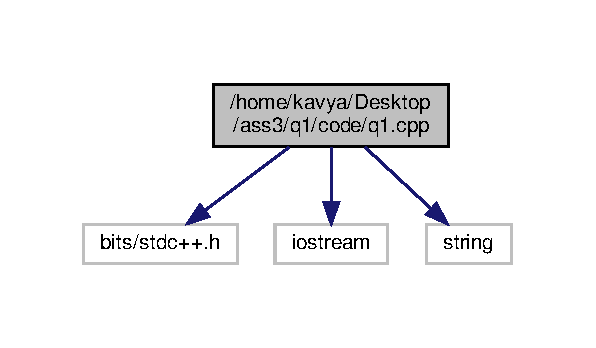
\includegraphics[width=286pt]{q1_8cpp__incl}
\end{center}
\end{figure}
\subsection*{Classes}
\begin{DoxyCompactItemize}
\item 
struct \hyperlink{struct_r_b_t_node}{R\+B\+T\+Node}
\begin{DoxyCompactList}\small\item\em \hyperlink{struct_r_b_t_node}{R\+B\+T\+Node} for red black tree. \end{DoxyCompactList}\item 
class \hyperlink{class_r_b_tree}{R\+B\+Tree}
\begin{DoxyCompactList}\small\item\em Class to represent Red-\/\+Black Tree. \end{DoxyCompactList}\item 
class \hyperlink{class_node}{Node}
\item 
class \hyperlink{class_a_v_l_tree}{A\+V\+L\+Tree}
\begin{DoxyCompactList}\small\item\em Class for A\+VL Tree. \end{DoxyCompactList}\item 
struct \hyperlink{structnode}{node}
\end{DoxyCompactItemize}
\subsection*{Enumerations}
\begin{DoxyCompactItemize}
\item 
enum \hyperlink{q1_8cpp_ab87bacfdad76e61b9412d7124be44c1c}{Color} \{ \hyperlink{q1_8cpp_ab87bacfdad76e61b9412d7124be44c1caf80f9a890089d211842d59625e561f88}{R\+ED}, 
\hyperlink{q1_8cpp_ab87bacfdad76e61b9412d7124be44c1caf77fb67151d0c18d397069ad8c271ba3}{B\+L\+A\+CK}
 \}
\end{DoxyCompactItemize}
\subsection*{Functions}
\begin{DoxyCompactItemize}
\item 
struct \hyperlink{structnode}{node} $\ast$ \hyperlink{q1_8cpp_a8a3ee315f73c586e51fcd202c4cd8662}{new\+Node} (int item)
\item 
void \hyperlink{q1_8cpp_a8e025ab1257df618068309e6a30fc93a}{inorder} (struct \hyperlink{structnode}{node} $\ast$root)
\item 
struct \hyperlink{structnode}{node} $\ast$ \hyperlink{q1_8cpp_a20a3b180a7700373071305e18971bb5e}{insert} (struct \hyperlink{structnode}{node} $\ast$\hyperlink{structnode}{node}, int key)
\item 
void \hyperlink{q1_8cpp_aa42e420e039d99993459c8d8a4fbdbdb}{print\+Path} (\hyperlink{structnode}{node} $\ast$rt, string s)
\item 
void \hyperlink{q1_8cpp_acfc11a0afabf3a77687b4b156d69cdd5}{get\+All\+Paths} (struct \hyperlink{structnode}{node} $\ast$\hyperlink{q1_8cpp_aab7df7514eae49d8d3b271504678bc75}{B\+ST})
\item 
void \hyperlink{q1_8cpp_a46640f831c90fba2fb20af78cea58a0c}{level\+Vise\+Indentation\+Helper} (\hyperlink{structnode}{node} $\ast$rt, int l)
\item 
void \hyperlink{q1_8cpp_a6e841fa6644d2916b88392bfcf8376d1}{level\+Vise\+Indentation} (\hyperlink{structnode}{node} $\ast$root)
\item 
void \hyperlink{q1_8cpp_aee650708cb84556644f8a4f6e7611c06}{create\+A\+V\+L\+Tree} (struct \hyperlink{structnode}{node} $\ast$rt)
\item 
int \hyperlink{q1_8cpp_ae66f6b31b5ad750f1fe042a706a4e3d4}{main} ()
\end{DoxyCompactItemize}
\subsection*{Variables}
\begin{DoxyCompactItemize}
\item 
\hyperlink{class_a_v_l_tree}{A\+V\+L\+Tree} \hyperlink{q1_8cpp_afa690420f01f46758f4ecfd9088af2b1}{A\+VL}
\item 
struct \hyperlink{structnode}{node} $\ast$ \hyperlink{q1_8cpp_aab7df7514eae49d8d3b271504678bc75}{B\+ST} = N\+U\+LL
\end{DoxyCompactItemize}


\subsection{Enumeration Type Documentation}
\mbox{\Hypertarget{q1_8cpp_ab87bacfdad76e61b9412d7124be44c1c}\label{q1_8cpp_ab87bacfdad76e61b9412d7124be44c1c}} 
\index{q1.\+cpp@{q1.\+cpp}!Color@{Color}}
\index{Color@{Color}!q1.\+cpp@{q1.\+cpp}}
\subsubsection{\texorpdfstring{Color}{Color}}
{\footnotesize\ttfamily enum \hyperlink{q1_8cpp_ab87bacfdad76e61b9412d7124be44c1c}{Color}}

\begin{DoxyEnumFields}{Enumerator}
\raisebox{\heightof{T}}[0pt][0pt]{\index{R\+ED@{R\+ED}!q1.\+cpp@{q1.\+cpp}}\index{q1.\+cpp@{q1.\+cpp}!R\+ED@{R\+ED}}}\mbox{\Hypertarget{q1_8cpp_ab87bacfdad76e61b9412d7124be44c1caf80f9a890089d211842d59625e561f88}\label{q1_8cpp_ab87bacfdad76e61b9412d7124be44c1caf80f9a890089d211842d59625e561f88}} 
R\+ED&\\
\hline

\raisebox{\heightof{T}}[0pt][0pt]{\index{B\+L\+A\+CK@{B\+L\+A\+CK}!q1.\+cpp@{q1.\+cpp}}\index{q1.\+cpp@{q1.\+cpp}!B\+L\+A\+CK@{B\+L\+A\+CK}}}\mbox{\Hypertarget{q1_8cpp_ab87bacfdad76e61b9412d7124be44c1caf77fb67151d0c18d397069ad8c271ba3}\label{q1_8cpp_ab87bacfdad76e61b9412d7124be44c1caf77fb67151d0c18d397069ad8c271ba3}} 
B\+L\+A\+CK&\\
\hline

\end{DoxyEnumFields}


Definition at line 6 of file q1.\+cpp.



\subsection{Function Documentation}
\mbox{\Hypertarget{q1_8cpp_aee650708cb84556644f8a4f6e7611c06}\label{q1_8cpp_aee650708cb84556644f8a4f6e7611c06}} 
\index{q1.\+cpp@{q1.\+cpp}!create\+A\+V\+L\+Tree@{create\+A\+V\+L\+Tree}}
\index{create\+A\+V\+L\+Tree@{create\+A\+V\+L\+Tree}!q1.\+cpp@{q1.\+cpp}}
\subsubsection{\texorpdfstring{create\+A\+V\+L\+Tree()}{createAVLTree()}}
{\footnotesize\ttfamily void create\+A\+V\+L\+Tree (\begin{DoxyParamCaption}\item[{struct \hyperlink{structnode}{node} $\ast$}]{rt }\end{DoxyParamCaption})}

This method will be used to create A\+VL Tree from in\+Order traversal of Binary Search Tree. 
\begin{DoxyParams}{Parameters}
{\em rt} & Root of the binary search tree(\+B\+S\+T). \\
\hline
\end{DoxyParams}
\begin{DoxyAuthor}{Author}
Kavya Barnwal 
\end{DoxyAuthor}
\begin{DoxyDate}{Date}
20/08/2019 
\end{DoxyDate}


Definition at line 770 of file q1.\+cpp.

\mbox{\Hypertarget{q1_8cpp_acfc11a0afabf3a77687b4b156d69cdd5}\label{q1_8cpp_acfc11a0afabf3a77687b4b156d69cdd5}} 
\index{q1.\+cpp@{q1.\+cpp}!get\+All\+Paths@{get\+All\+Paths}}
\index{get\+All\+Paths@{get\+All\+Paths}!q1.\+cpp@{q1.\+cpp}}
\subsubsection{\texorpdfstring{get\+All\+Paths()}{getAllPaths()}}
{\footnotesize\ttfamily void get\+All\+Paths (\begin{DoxyParamCaption}\item[{struct \hyperlink{structnode}{node} $\ast$}]{B\+ST }\end{DoxyParamCaption})}

This method will be used to print all the paths from root node to the N\+U\+LL pointers. 
\begin{DoxyParams}{Parameters}
{\em B\+ST} & Root of B\+ST. \\
\hline
\end{DoxyParams}
\begin{DoxyAuthor}{Author}
Kavya Barnwal 
\end{DoxyAuthor}
\begin{DoxyDate}{Date}
20/08/2019 
\end{DoxyDate}


Definition at line 721 of file q1.\+cpp.

\mbox{\Hypertarget{q1_8cpp_a8e025ab1257df618068309e6a30fc93a}\label{q1_8cpp_a8e025ab1257df618068309e6a30fc93a}} 
\index{q1.\+cpp@{q1.\+cpp}!inorder@{inorder}}
\index{inorder@{inorder}!q1.\+cpp@{q1.\+cpp}}
\subsubsection{\texorpdfstring{inorder()}{inorder()}}
{\footnotesize\ttfamily void inorder (\begin{DoxyParamCaption}\item[{struct \hyperlink{structnode}{node} $\ast$}]{root }\end{DoxyParamCaption})}

A utility function to do inorder traversal of B\+ST. 
\begin{DoxyParams}{Parameters}
{\em node} & Root of B\+ST. \\
\hline
{\em key} & data to be inserted. \\
\hline
\end{DoxyParams}
\begin{DoxyAuthor}{Author}
Kavya Barnwal 
\end{DoxyAuthor}
\begin{DoxyDate}{Date}
20/08/2019 
\end{DoxyDate}


Definition at line 659 of file q1.\+cpp.

\mbox{\Hypertarget{q1_8cpp_a20a3b180a7700373071305e18971bb5e}\label{q1_8cpp_a20a3b180a7700373071305e18971bb5e}} 
\index{q1.\+cpp@{q1.\+cpp}!insert@{insert}}
\index{insert@{insert}!q1.\+cpp@{q1.\+cpp}}
\subsubsection{\texorpdfstring{insert()}{insert()}}
{\footnotesize\ttfamily struct \hyperlink{structnode}{node}$\ast$ insert (\begin{DoxyParamCaption}\item[{struct \hyperlink{structnode}{node} $\ast$}]{node,  }\item[{int}]{key }\end{DoxyParamCaption})}

A utility function to insert a new node with given key in B\+ST. 
\begin{DoxyParams}{Parameters}
{\em node} & Root of B\+ST. \\
\hline
{\em key} & data to be inserted. \\
\hline
\end{DoxyParams}
\begin{DoxyAuthor}{Author}
Kavya Barnwal 
\end{DoxyAuthor}
\begin{DoxyDate}{Date}
20/08/2019 
\end{DoxyDate}


Definition at line 676 of file q1.\+cpp.

\mbox{\Hypertarget{q1_8cpp_a6e841fa6644d2916b88392bfcf8376d1}\label{q1_8cpp_a6e841fa6644d2916b88392bfcf8376d1}} 
\index{q1.\+cpp@{q1.\+cpp}!level\+Vise\+Indentation@{level\+Vise\+Indentation}}
\index{level\+Vise\+Indentation@{level\+Vise\+Indentation}!q1.\+cpp@{q1.\+cpp}}
\subsubsection{\texorpdfstring{level\+Vise\+Indentation()}{levelViseIndentation()}}
{\footnotesize\ttfamily void level\+Vise\+Indentation (\begin{DoxyParamCaption}\item[{\hyperlink{structnode}{node} $\ast$}]{root }\end{DoxyParamCaption})}

This method will be used to print the Binary Search Tree(\+B\+S\+T) with lavel-\/wise-\/indentation. 
\begin{DoxyParams}{Parameters}
{\em root} & Root of B\+ST. \\
\hline
\end{DoxyParams}
\begin{DoxyAuthor}{Author}
Kavya Barnwal 
\end{DoxyAuthor}
\begin{DoxyDate}{Date}
20/08/2019 
\end{DoxyDate}


Definition at line 759 of file q1.\+cpp.

\mbox{\Hypertarget{q1_8cpp_a46640f831c90fba2fb20af78cea58a0c}\label{q1_8cpp_a46640f831c90fba2fb20af78cea58a0c}} 
\index{q1.\+cpp@{q1.\+cpp}!level\+Vise\+Indentation\+Helper@{level\+Vise\+Indentation\+Helper}}
\index{level\+Vise\+Indentation\+Helper@{level\+Vise\+Indentation\+Helper}!q1.\+cpp@{q1.\+cpp}}
\subsubsection{\texorpdfstring{level\+Vise\+Indentation\+Helper()}{levelViseIndentationHelper()}}
{\footnotesize\ttfamily void level\+Vise\+Indentation\+Helper (\begin{DoxyParamCaption}\item[{\hyperlink{structnode}{node} $\ast$}]{rt,  }\item[{int}]{l }\end{DoxyParamCaption})}

Helper method for method \hyperlink{q1_8cpp_a6e841fa6644d2916b88392bfcf8376d1}{level\+Vise\+Indentation()}. 
\begin{DoxyParams}{Parameters}
{\em root} & Root of B\+ST. \\
\hline
{\em l} & level of that node. \\
\hline
\end{DoxyParams}
\begin{DoxyAuthor}{Author}
Kavya Barnwal 
\end{DoxyAuthor}
\begin{DoxyDate}{Date}
20/08/2019 
\end{DoxyDate}


Definition at line 738 of file q1.\+cpp.

\mbox{\Hypertarget{q1_8cpp_ae66f6b31b5ad750f1fe042a706a4e3d4}\label{q1_8cpp_ae66f6b31b5ad750f1fe042a706a4e3d4}} 
\index{q1.\+cpp@{q1.\+cpp}!main@{main}}
\index{main@{main}!q1.\+cpp@{q1.\+cpp}}
\subsubsection{\texorpdfstring{main()}{main()}}
{\footnotesize\ttfamily int main (\begin{DoxyParamCaption}{ }\end{DoxyParamCaption})}



Definition at line 781 of file q1.\+cpp.

\mbox{\Hypertarget{q1_8cpp_a8a3ee315f73c586e51fcd202c4cd8662}\label{q1_8cpp_a8a3ee315f73c586e51fcd202c4cd8662}} 
\index{q1.\+cpp@{q1.\+cpp}!new\+Node@{new\+Node}}
\index{new\+Node@{new\+Node}!q1.\+cpp@{q1.\+cpp}}
\subsubsection{\texorpdfstring{new\+Node()}{newNode()}}
{\footnotesize\ttfamily struct \hyperlink{structnode}{node}$\ast$ new\+Node (\begin{DoxyParamCaption}\item[{int}]{item }\end{DoxyParamCaption})}

A utility function to create a new B\+ST node. 
\begin{DoxyParams}{Parameters}
{\em item} & data to be inserted. \\
\hline
\end{DoxyParams}
\begin{DoxyAuthor}{Author}
Kavya Barnwal 
\end{DoxyAuthor}
\begin{DoxyDate}{Date}
20/08/2019 
\end{DoxyDate}


Definition at line 644 of file q1.\+cpp.

\mbox{\Hypertarget{q1_8cpp_aa42e420e039d99993459c8d8a4fbdbdb}\label{q1_8cpp_aa42e420e039d99993459c8d8a4fbdbdb}} 
\index{q1.\+cpp@{q1.\+cpp}!print\+Path@{print\+Path}}
\index{print\+Path@{print\+Path}!q1.\+cpp@{q1.\+cpp}}
\subsubsection{\texorpdfstring{print\+Path()}{printPath()}}
{\footnotesize\ttfamily void print\+Path (\begin{DoxyParamCaption}\item[{\hyperlink{structnode}{node} $\ast$}]{rt,  }\item[{string}]{s }\end{DoxyParamCaption})}

Helper method for method \hyperlink{q1_8cpp_acfc11a0afabf3a77687b4b156d69cdd5}{get\+All\+Paths()}. 
\begin{DoxyParams}{Parameters}
{\em rt} & Root of B\+ST. \\
\hline
{\em s} & string containing details of nodes traversed. \\
\hline
\end{DoxyParams}
\begin{DoxyAuthor}{Author}
Kavya Barnwal 
\end{DoxyAuthor}
\begin{DoxyDate}{Date}
20/08/2019 
\end{DoxyDate}


Definition at line 699 of file q1.\+cpp.



\subsection{Variable Documentation}
\mbox{\Hypertarget{q1_8cpp_afa690420f01f46758f4ecfd9088af2b1}\label{q1_8cpp_afa690420f01f46758f4ecfd9088af2b1}} 
\index{q1.\+cpp@{q1.\+cpp}!A\+VL@{A\+VL}}
\index{A\+VL@{A\+VL}!q1.\+cpp@{q1.\+cpp}}
\subsubsection{\texorpdfstring{A\+VL}{AVL}}
{\footnotesize\ttfamily \hyperlink{class_a_v_l_tree}{A\+V\+L\+Tree} A\+VL}



Definition at line 628 of file q1.\+cpp.

\mbox{\Hypertarget{q1_8cpp_aab7df7514eae49d8d3b271504678bc75}\label{q1_8cpp_aab7df7514eae49d8d3b271504678bc75}} 
\index{q1.\+cpp@{q1.\+cpp}!B\+ST@{B\+ST}}
\index{B\+ST@{B\+ST}!q1.\+cpp@{q1.\+cpp}}
\subsubsection{\texorpdfstring{B\+ST}{BST}}
{\footnotesize\ttfamily struct \hyperlink{structnode}{node}$\ast$ B\+ST = N\+U\+LL}



Definition at line 636 of file q1.\+cpp.


%--- End generated contents ---

% Index
\backmatter
\newpage
\phantomsection
\clearemptydoublepage
\addcontentsline{toc}{chapter}{Index}
\printindex

\end{document}
